\documentclass[11pt]{article}

% Change "review" to "final" to generate the camera-ready version.
% Change to "preprint" to generate a non-anonymous version with page numbers.
\usepackage[review]{acl}

\usepackage{times}
\usepackage{latexsym}
\usepackage[T1]{fontenc}
\usepackage[utf8]{inputenc}
\usepackage{microtype}
\usepackage{inconsolata}
\usepackage{graphicx}
\usepackage{amsmath}
\usepackage{amssymb}
\usepackage{booktabs}
\usepackage{tabularx}
\usepackage{array}
\usepackage{xcolor}
\usepackage{tikz}
\usepackage{pgfplots}
\pgfplotsset{compat=1.18}
\usetikzlibrary{arrows.meta,positioning,shapes.geometric,fit}

\newcommand{\pimplanbench}{\textsc{PIM-PlanBench}}
\newcommand{\planscore}{\textsc{PlanScore}}
\newcommand{\pwg}{\textsc{Physics Workflow Graph}}
\newcommand{\verifier}{\textsc{Verifier}}
\newcommand{\facetset}{\mathcal{F}}
\newcommand{\taskset}{\mathcal{T}}
\newcommand{\modelset}{\mathcal{M}}

\title{\pimplanbench{}: Evaluating Planning-Stage Reasoning for Physics-Informed Modeling}

\author{Anonymous EMNLP submission}

\begin{document}
\maketitle

\begin{abstract}
Physics-informed modeling depends on a planning layer that precedes implementation: a natural-language problem must be converted into variables, constraints, model choices, losses, and validation checks before code or numerical training can be meaningful. Existing evaluations of scientific language models often emphasize final answers, tool use, or executable code, and therefore under-specify whether a model can make these model-design decisions. We introduce \pimplanbench{}, a compact benchmark for evaluating planning-stage reasoning in physics-informed modeling. The benchmark contains 26 natural-language tasks spanning heat transfer, wave propagation, transport, fluid dynamics, phase-field modeling, porous media, magnetohydrodynamics, acoustics, and related domains. Each task pairs a public model-facing prompt with a private reference and a five-facet \planscore{} rubric covering problem formalization, physics constraints, model choice, training strategy, and validation or failure risks. To separate task-specific planning from generic PINN recipes, \planscore{} v0.3 adds critical points and cap rules for hallucinated specifications, missing constraints, wrong task type, and hard-trap cases such as shocks, high-frequency Helmholtz problems, multiscale Darcy flow, Cahn-Hilliard dynamics, and divergence-controlled magnetohydrodynamics. In a direct-planner pilot over six contemporary language models, all models produce schema-valid plans for all 26 tasks, but deterministic first-pass scores reveal substantial saturation: 297 of 780 facet scores reach the ceiling and 14 tasks have low model separation. A 180-row human calibration subset yields a mean absolute human-auto difference of 0.442, indicating that automatic scoring is useful for screening and audit preparation but should not replace adjudication for paper-facing claims. \pimplanbench{} provides task files, private references, scoring scripts, and review workbooks for studying whether language models can reason about physics-informed modeling before execution begins.
\end{abstract}

\section{Introduction}

Physics-informed modeling begins with model-design choices that are made before any executable solver exists. A natural-language problem must be translated into state variables, known inputs, missing specifications, governing residuals, boundary and initial conditions, admissible model classes, loss terms, and validation checks. This translation is a planning problem: a smooth, fully specified PDE may admit a standard physics-informed neural network (PINN), whereas shocks, high-frequency fields, sparse observations, coupled variables, or divergence constraints may require weak formulations, conservative objectives, neural operators, domain decomposition, or hybrid numerical-neural workflows. Evaluating this planning layer is therefore necessary for understanding whether language models can support physics-informed modeling, rather than merely produce plausible solver code or generic PINN recipes.

These decisions define an intermediate reasoning stage between natural-language problem understanding and executable numerical modeling. Existing evaluations of LLMs for scientific work often measure end-to-end task completion, tool use, code execution, data-driven discovery, or hypothesis generation \citep{flowbench2024,scienceagentbench2025,discoverybench2024,agentsthatmatter2024}. Such benchmarks are essential, but they can obscure whether a failure comes from syntax, environment setup, optimization instability, missing domain knowledge, or an invalid modeling plan. Physics-informed modeling exposes this gap sharply: a fluent generic PINN recipe can look plausible while omitting the exact constraints that make a problem physically meaningful.

We propose \pimplanbench{}, a benchmark for evaluating planning-stage reasoning in physics-informed modeling. The model-facing input is a natural-language physics problem. The expected output is a structured plan with five sections: problem formalization, physics constraints, model choice, training strategy, and validation or failure risks. The benchmark does not directly reward final PDE solver accuracy. Instead, it asks whether a model can construct a scientifically valid and operational modeling plan before implementation.

The current v0.3 release contains 26 public tasks and private scoring references. Tasks span easy forward PDE examples, medium inverse or sparse-observation problems, hard stiffness and high-frequency cases, and hard-plus stress tasks designed to expose generic reasoning. The scoring protocol uses a 0--5 scale for each of five facets, giving 25 points per task. Private references include critical points, failure traps, and cap rules that limit scores for generic PINN workflows, unsupported assumptions, missing observations, wrong task type, or validation based only on generic MSE.

Our pilot evaluation runs a direct-planner prompt over six models and scores 780 facet-level outputs. The results show that current models can produce complete structured plans, but they also reveal saturation and incomplete task-level discrimination. These findings motivate two uses of \pimplanbench{}: as a resource for measuring planning-stage scientific reasoning, and as a diagnostic loop for designing harder task variants and sharper rubrics.

Our contributions are:
\begin{itemize}
    \item We define physics-informed model-design planning as an evaluation target between natural-language problem understanding and executable solver construction.
    \item We release a 26-task benchmark with public model-facing tasks and private scoring references for physics-informed modeling plans.
    \item We introduce \planscore{} v0.3, a five-facet 0--5 rubric with explicit cap rules for generic workflows, hallucinated specifications, missing physical constraints, and hard-trap cases.
    \item We provide an auditable evaluation pipeline: JSONL task files, model runners, normalization, facet-row construction, deterministic first-pass scoring, HTML reports, and human-review workbooks.
    \item We report a direct-planner pilot over six models and analyze score coverage, saturation, model separation, and human-auto calibration on a 180-row subset.
\end{itemize}

\section{Related Work}

\paragraph{LLM agents and workflow planning.}
LLM agents commonly interleave reasoning, tool use, and feedback \citep{react2023}. Chain-of-thought prompting improves multi-step reasoning in language models \citep{wei2022cot}, but free-form reasoning can be brittle when domain constraints are implicit. FlowBench revisits workflow-guided planning for LLM-based agents \citep{flowbench2024}. \pimplanbench{} shares the view that workflows are first-class evaluation objects, but specializes the target to physics-informed model-design planning rather than general tool sessions.

\paragraph{Scientific discovery agents.}
ScienceAgentBench evaluates agents on data-driven scientific discovery tasks extracted from peer-reviewed papers \citep{scienceagentbench2025}. DiscoveryBench studies data-driven hypothesis discovery with LLMs \citep{discoverybench2024}. Agent Laboratory investigates autonomous research pipelines from idea to report \citep{agentlaboratory2025}. These benchmarks motivate rigorous evaluation of scientific agents, while \pimplanbench{} isolates a narrower capability: the quality of the modeling plan before code generation and long training runs.

\paragraph{Physics-informed modeling and PDE benchmarks.}
PINNs embed governing equations into neural-network objectives and support forward and inverse PDE problems \citep{raissi2019pinn}. DeepXDE provides a practical library for differential-equation learning \citep{lu2021deepxde}, and broader surveys discuss physics-informed machine learning applications and limitations \citep{karniadakis2021physics}. PINNacle offers a diverse benchmark for PINN methods across PDE families and difficulty factors \citep{pinnacle2024}. The Well provides large-scale physics simulations for machine-learning evaluation \citep{thewell2024}. These resources mainly evaluate solvers, models, or simulation fields; \pimplanbench{} evaluates natural-language planning artifacts.

\paragraph{Language agents for PDE and PINN systems.}
Lang-PINN turns natural-language descriptions into trainable PINN code through a multi-agent framework \citep{langpinn2025}. PDE-Agent frames PDE solving as tool invocation by a multi-agent framework \citep{pdeagent2025}. PDE-Controller studies LLM autoformalization and reasoning for PDE control \citep{pdecontroller2025}. Our benchmark is complementary: it evaluates whether the plan itself contains the mathematical and operational decisions needed before such systems are executed.

\section{Benchmark}

\subsection{Task Definition}

Each benchmark item is formulated as a natural-language physics-informed modeling request. Under a unified prompting protocol, the model receives the public task description and the corresponding planning instruction, and must return exactly one JSON object with five sections:
\begin{enumerate}
    \item \textbf{Problem Formalization}: variables, domain, known and unknown quantities, task type, and objective.
    \item \textbf{Physics Constraints}: PDE residuals, initial conditions, boundary conditions, observations, conservation laws, symmetries, units, and admissible ranges.
    \item \textbf{Model Choice}: model family, inputs, outputs, architecture, and task-specific justification.
    \item \textbf{Training Strategy}: loss terms, weighting, sampling, optimization, normalization, curricula, and stopping criteria.
    \item \textbf{Validation Failure Risks}: metrics, physics checks, baselines, failure modes, and reproducibility notes.
\end{enumerate}

A separate private reference set is withheld from model access. It records the canonical PDE formulation, expected variables, physical constraints, admissible modeling choices, expected loss components, validation checks, critical points, cap rules, scoring tags, and review flags. This public/private separation reduces leakage risk while preserving an auditable scoring contract.

\subsection{Task Set}

The v0.3 benchmark contains 26 tasks: 7 easy, 8 medium, 5 hard, and 6 hard-plus items. Tasks cover 19 task types and 13 domains, including heat transfer, wave propagation, transport, fluid dynamics, potential fields, phase-field modeling, porous media, acoustics, compressible flow, magnetohydrodynamics, thermal-fluid dynamics, chemical biology, and wave physics. Figure~\ref{fig:task-composition} summarizes the difficulty distribution, Table~\ref{tab:task-examples} gives representative examples, and Appendix~\ref{app:task-inventory} lists the complete task inventory.

\begin{table*}[t]
\caption{Representative \pimplanbench{} v0.3 tasks. The benchmark is compact by design, but it spans forward solves, inverse problems, sparse observations, missing-condition handling, high-frequency settings, discontinuities, and coupled constrained fields.}
\label{tab:task-examples}
\centering
\small
\begin{tabularx}{\textwidth}{p{0.15\textwidth}p{0.22\textwidth}p{0.22\textwidth}X}
\toprule
\textbf{Difficulty} & \textbf{Task type} & \textbf{PDE/system} & \textbf{Planning challenge} \\
\midrule
Easy & Forward PDE solving & 1D heat equation & Identify the temperature field, heat residual, IC/BC losses, and analytic or numerical validation. \\
Medium & Inverse parameter estimation & Viscous Burgers equation & Separate known observations from unknown viscosity and include data misfit plus identifiability checks. \\
Medium & Periodic constraint handling & Advection-diffusion equation & Enforce periodic compatibility beyond endpoint value matching, including derivative or flux consistency. \\
Hard & High-frequency modeling & Helmholtz equation & Address complex-valued fields, phase error, points-per-wavelength sampling, and spectral bias. \\
Hard & High-order PDE modeling & Cahn-Hilliard equation & Use chemical-potential or mixed-form reasoning and validate mass conservation and energy drift. \\
Hard-plus & Discontinuous solution modeling & Compressible Euler shocks & Avoid smooth pointwise residuals alone; use weak, conservative, or shock-aware treatment. \\
Hard-plus & Coupled constrained fields & Resistive magnetohydrodynamics & Model coupled velocity and magnetic induction while controlling magnetic divergence. \\
Hard-plus & Multiscale operator or solver design & High-contrast Darcy flow & Distinguish a single high-contrast solve from reusable operator learning over coefficient fields. \\
\bottomrule
\end{tabularx}
\end{table*}

\begin{figure}[t]
\centering
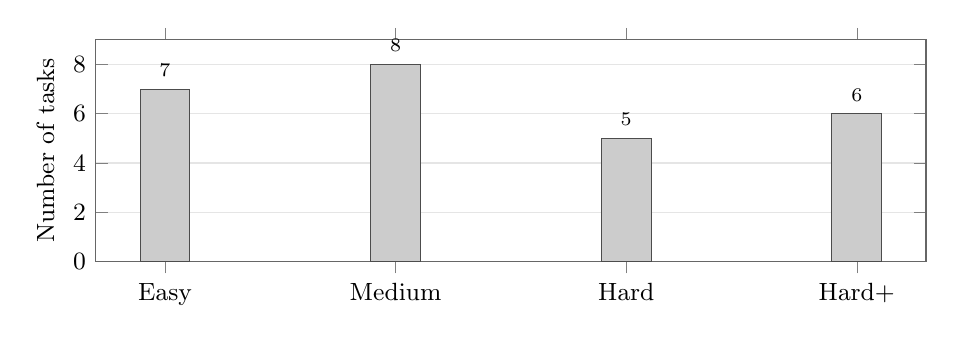
\begin{tikzpicture}
\begin{axis}[
     ybar,
    width=\columnwidth,
    height=4.4cm,
    ymin=0,
    ymax=9,
    ylabel={Number of tasks},
    symbolic x coords={Easy,Medium,Hard,Hard+},
    xtick=data,
    nodes near coords,
    every node near coord/.append style={
        font=\scriptsize,
        yshift=1pt
    },
    bar width=18pt,
    tick label style={font=\small},
    label style={font=\small},
    ymajorgrids=true,
    grid style={gray!20},
    axis line style={black!60}
]
\addplot[fill=black!20,draw=black!70] coordinates {(Easy,7) (Medium,8) (Hard,5) (Hard+,6)};
\end{axis}
\end{tikzpicture}
\caption{Task composition by difficulty in the current v0.3 release. The hard-plus split is reserved for stress cases where generic PINN templates should not receive full credit.}
\label{fig:task-composition}
\end{figure}

\subsection{Hard-Trap Design}

The v0.3 revision intentionally reduces method leakage in public prompts and tightens private scoring references. The hard-trap tasks require a central modeling decision rather than a longer generic answer. For example, the Euler shock task requires conservative variables and weak, integral, finite-volume, or otherwise shock-aware treatment. The high-frequency Helmholtz task requires complex or phase-aware reasoning and sampling that scales with wavelength. The Cahn-Hilliard task requires chemical-potential or mixed-form reasoning and conservation checks. The MHD task requires magnetic divergence control rather than an unexamined soft penalty. These cases are designed to separate domain-grounded planning from fluent template completion.

\section{\planscore{} v0.3}

\subsection{Facet Rubric}

Each answer is scored on five facets, summarized in Table~\ref{tab:facets}. Let $\facetset$ be the facet set and let
\[
\facetset = \{\mathrm{PF}, \mathrm{PC}, \mathrm{MC}, \mathrm{TS}, \mathrm{VR}\},
\]
where PF is problem formalization, PC is physics constraints, MC is model choice, TS is training strategy, and VR is validation and failure risks. For model $m \in \modelset$, task $t \in \taskset$, and facet $f \in \facetset$, the final facet score is
\[
s_{m,t,f} \in \{0,1,2,3,4,5\}.
\]
The task score and model-level average are
\begin{align}
S_{m,t} &= \sum_{f \in \facetset} s_{m,t,f}, \qquad 0 \le S_{m,t} \le 25, \\
\bar{S}_{m} &= \frac{1}{|\taskset|}\sum_{t \in \taskset} S_{m,t}.
\end{align}

\begin{table}[t]
\caption{Five \planscore{} facets. The rubric reports the facets separately because different models can fail in different stages of a physics-informed workflow.}
\label{tab:facets}
\centering
\small
\begin{tabularx}{\columnwidth}{p{0.25\columnwidth}X}
\toprule
\textbf{Facet} & \textbf{Scoring focus} \\
\midrule
Problem Formalization & Unknowns, known inputs, task type, domain, missing specifications, and objective. \\
Physics Constraints & Governing residuals, IC/BC/data terms, conservation laws, compatibility conditions, and task-specific physics. \\
Model Choice & Architecture or method justified by PDE type, data regime, constraints, and failure modes. \\
Training Strategy & Losses, sampling, optimization, weighting, normalization, and stability measures. \\
Validation Failure Risks & Physical validation metrics, diagnostics, baselines, and task-specific failure modes. \\
\bottomrule
\end{tabularx}
\end{table}

The scale is deliberately ordinal. A score of 0 denotes a missing, irrelevant, or physically wrong answer. Scores 1--2 denote broad recognition or partial correctness with major omissions. Scores 3--4 denote mostly correct task-specific planning with increasing operational detail. A 5 requires task-specific correctness, an executable workflow, and no triggered cap rule. Appendix~\ref{app:rubric-details} gives additional rubric details and cap-rule examples.

\subsection{Automatic First-Pass Scoring}

The current repository implements a deterministic automated scoring system for first-pass evaluation. It is designed to support screening, visualization, and audit preparation, rather than to serve as a substitute for final human adjudication.

For each answer span $a_{m,t,f}$, the scorer computes a reference-item match ratio and a facet-cue coverage ratio. Let $R_{t,f}$ be the private reference items for task $t$ and facet $f$, including critical points plus facet-specific fields such as acceptable model choices, expected loss terms, validation checks, and failure traps. Let $q(a,r)$ indicate whether answer $a$ matches reference item $r$ under normalized token and synonym matching. The reference specificity term is
\begin{equation}
\rho_{m,t,f} =
\frac{1}{|R_{t,f}|}\sum_{r \in R_{t,f}} \mathbb{1}[q(a_{m,t,f}, r)] .
\end{equation}
Let $C_f$ be the facet cue list and let $g(a,c)$ indicate whether cue $c$ appears in $a$. The cue coverage term is capped at five cues:
\begin{equation}
\kappa_{m,t,f} =
\min\left(1, \frac{\sum_{c \in C_f} \mathbb{1}[g(a_{m,t,f},c)]}{\min(5,|C_f|)}\right).
\end{equation}
The raw automatic score is a rounded and clipped function of specificity, cue coverage, answer length, missing-information handling, and high-detail bonuses:

\begin{equation}
\begin{aligned}
r_{m,t,f}
= \mathrm{clip}_{0,5}\Bigg(
\mathrm{round}\Big[
&1 + 2.2\rho_{m,t,f} \\
&+ 1.25\min\left(\frac{\kappa_{m,t,f}}{0.45},1\right) \\
&+ b(a_{m,t,f})
\Big]\Bigg).
\end{aligned}
\end{equation}


where $b(a)$ collects small deterministic bonuses for sufficient detail, explicitly flagged missing information, and high reference coverage. This formulation intentionally rewards both reference overlap and operational specificity while keeping the maximum bounded.

\subsection{Cap Rules}

The most important part of \planscore{} is not the raw matching function but the cap mechanism. Private references and the rubric define conditions under which a plausible answer cannot receive full credit. Let $\mathcal{A}_{t,f}(a)$ be the set of active cap rules for answer $a$ on task $t$ and facet $f$, and let $\gamma(h)$ be the maximum allowed score under cap rule $h$. The final automatic score is
\begin{equation}
s_{m,t,f} =
\min\left(r_{m,t,f},\ \min_{h \in \mathcal{A}_{t,f}(a_{m,t,f})} \gamma(h)\right),
\label{eq:cap}
\end{equation}
with the inner minimum set to 5 when no cap is active. Equation~\ref{eq:cap} encodes the benchmark's core evaluation philosophy: generic breadth should not override missing task-specific physics. Examples include capping a generic PINN template at 3, capping hallucinated IC/BC or parameter values at 2 on affected facets, capping a Helmholtz answer that treats the task as time-domain wave propagation at 2 for problem formalization and physics constraints, and capping MHD answers without magnetic divergence control at 2 on affected facets.

\begin{figure*}[t]
\centering
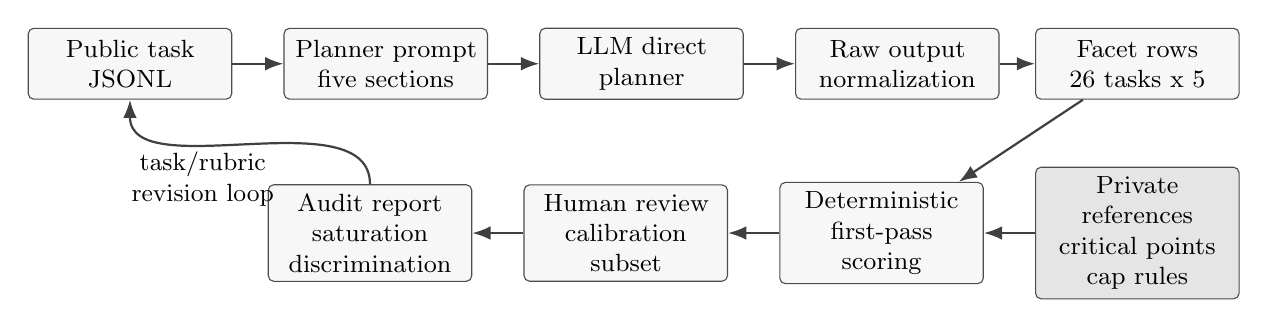
\begin{tikzpicture}[
    node distance=0.95cm and 0.65cm,
    box/.style={
        draw=black!70,
        rounded corners=2pt,
        align=center,
        minimum width=2.45cm,
        minimum height=0.9cm,
        text width=2.35cm,
        font=\small,
        fill=black!3
    },
    priv/.style={
        draw=black!70,
        rounded corners=2pt,
        align=center,
        minimum width=2.45cm,
        minimum height=0.9cm,
        text width=2.35cm,
        font=\small,
        fill=black!10
    },
    arrow/.style={-Latex, thick, draw=black!75}
]
\node[box] (task) {Public task\\JSONL};
\node[box, right=of task] (prompt) {Planner prompt\\five sections};
\node[box, right=of prompt] (model) {LLM direct\\planner};
\node[box, right=of model] (norm) {Raw output\\normalization};

\node[box, right=0.45cm of norm] (rows) {Facet rows\\26 tasks x 5};

\node[priv, below=0.85cm of rows] (refs) {Private references\\critical points\\cap rules};

\node[box, left=of refs] (score) {Deterministic\\first-pass scoring};
\node[box, left=of score] (human) {Human review\\calibration subset};
\node[box, left=of human] (audit) {Audit report\\saturation\\discrimination};

\draw[arrow] (task) -- (prompt);
\draw[arrow] (prompt) -- (model);
\draw[arrow] (model) -- (norm);
\draw[arrow] (norm) -- (rows);
\draw[arrow] (rows) -- (score);
\draw[arrow] (refs) -- (score);
\draw[arrow] (score) -- (human);
\draw[arrow] (human) -- (audit);

\draw[arrow] 
    (audit.north) .. controls +(0,1.1) and +(0,-1.1) ..
    node[below,font=\small,align=center,xshift=-6mm] {task/rubric\\revision loop}
    (task.south);

\end{tikzpicture}
\caption{Evaluation pipeline. Public tasks and the planner prompt generate normalized model plans, which are converted into facet rows. Private references supply critical points and cap rules for deterministic first-pass scoring. Manual review calibrates the automatic scores and identifies saturation or low-discrimination tasks for the next benchmark revision.}
\label{fig:pipeline}
\end{figure*}

\subsection{Diagnostic Metrics}

Beyond model averages, \pimplanbench{} reports metrics that expose whether the benchmark is discriminative. The ceiling rate at threshold $\tau$ is

\begin{equation}
\begin{aligned}
\mathrm{Ceil}_{\tau}
&=
\frac{1}{|\modelset||\taskset||\facetset|} \\
&\quad \times
\sum_{m,t,f}\mathbb{1}[s_{m,t,f}\ge \tau].
\end{aligned}
\end{equation}

Task-level model separation is


\begin{equation}
\Delta_t = \max_{m \in \modelset} S_{m,t} - \min_{m \in \modelset} S_{m,t}.
\end{equation}

A low $\Delta_t$ identifies tasks that may be too easy, too generic, or insufficiently constrained by their private references. For human calibration, let $h_i$ and $a_i$ be human and automatic scores for comparable row $i$. We report
\begin{align}
\mathrm{MAE} &= \frac{1}{n}\sum_{i=1}^{n}|h_i-a_i|, \\
\mathrm{Within}_{\epsilon} &= \frac{1}{n}\sum_{i=1}^{n}\mathbb{1}[|h_i-a_i|\le \epsilon].
\end{align}
These metrics support the paper's bounded claim: automatic scores are useful for screening and audit preparation, while final paper-facing claims should be checked by human adjudication.

\section{Evaluation Setup}

\subsection{Pipeline}

The repository implements the pipeline in Figure~\ref{fig:pipeline}. The runner renders the canonical prompt and writes raw plus normalized outputs under \texttt{runs/pilot\_v0.3/}. A row builder converts normalized outputs into facet-level CSV rows. The deterministic scorer assigns first-pass scores and rationales. A visualization script creates HTML reports. Manual-scoring scripts build review workbooks, and a comparison script joins manual rows with automatic scores.

The pipeline separates public tasks from private references throughout. This separation is important for benchmark credibility: the model sees only the information it should reason from, while the private references preserve hidden scoring details, acceptable alternatives, failure traps, and cap rules.

\subsection{Models}

The v0.3 direct-planner pilot contains normalized outputs for six models: moonshotai/Kimi-K2.6, zai-org/GLM-4.7, zai-org/GLM-5.1, DeepSeek-V4-Flash, deepseek-v4-pro, and qwen3.7-max. All six models produce valid normalized outputs for all 26 public tasks and all five facets, yielding 780 scored rows.

The evaluated systems are accessed through hosted OpenAI-compatible APIs rather than trained or served locally. We therefore report the computational budget at the request level, and we do not report local GPU hours. Provider-side parameter counts, active-parameter counts, and serving infrastructure are not consistently available for all API models.

\subsection{Inference Configuration}

All direct-planner runs use the same OpenAI-compatible chat-completions runner and the same canonical v0.3 prompt. Table~\ref{tab:api-config} reports the decoding and request-control parameters used for the API calls. These settings are part of the evaluation protocol because decoding randomness, token budget, and retry behavior can affect schema validity, plan completeness, and downstream facet scores.

\begin{table}[t]
\caption{API inference configuration used for the v0.3 direct-planner pilot.}
\label{tab:api-config}
\centering
\small
\begin{tabularx}{\columnwidth}{l r X}
\toprule
\textbf{Parameter} & \textbf{Value} & \textbf{Role in evaluation} \\
\midrule
Temperature & 0.2 & Low-variance decoding to reduce stochastic differences across repeated calls. \\
Max tokens & 1800 & Output budget for producing the five-section structured plan. \\
Timeout & 120 s & Per-request timeout for provider API calls. \\
Retries & 2 & Number of retry attempts after transient API failures. \\
\bottomrule
\end{tabularx}
\end{table}

  
\section{Results}

\subsection{Overall Scores}

Table~\ref{tab:model-scores} reports deterministic first-pass scores, and Figure~\ref{fig:model-bars} visualizes average task scores. These numbers should be read as pilot evidence, not as final leaderboard claims. The best current average is Kimi-K2.6 with 22.154 out of 25 points per task. The spread between the top model and the lowest-scoring model is 2.231 points per task, which is meaningful for diagnostic analysis but small enough that model-ranking claims should remain conservative.

\begin{table*}[t]
\caption{Direct-planner pilot results on 26 tasks. Scores are deterministic first-pass \planscore{} values from the v0.3 scorer and should be interpreted with the human-calibration results in Table~\ref{tab:manual-auto}.}
\label{tab:model-scores}
\centering
\small
\begin{tabular}{lrrrrrrr}
\toprule
\textbf{Model} & \textbf{Rows} & \textbf{Total} & \textbf{Avg facet} & \textbf{Avg task} & \textbf{PF} & \textbf{PC} & \textbf{VR} \\
\midrule
Kimi-K2.6 & 130 & 576.0 & 4.431 & 22.154 & 4.385 & 4.231 & 4.346 \\
GLM-5.1 & 130 & 567.0 & 4.362 & 21.808 & 4.038 & 4.269 & 4.385 \\
qwen3.7-max & 130 & 551.0 & 4.238 & 21.192 & 4.192 & 4.077 & 4.000 \\
DeepSeek-V4-Flash & 130 & 549.0 & 4.223 & 21.115 & 4.077 & 4.154 & 3.962 \\
deepseek-v4-pro & 130 & 549.0 & 4.223 & 21.115 & 4.231 & 4.000 & 4.115 \\
GLM-4.7 & 130 & 518.0 & 3.985 & 19.923 & 4.000 & 3.808 & 4.077 \\
\bottomrule
\end{tabular}
\end{table*}

\begin{figure}[t]
\centering
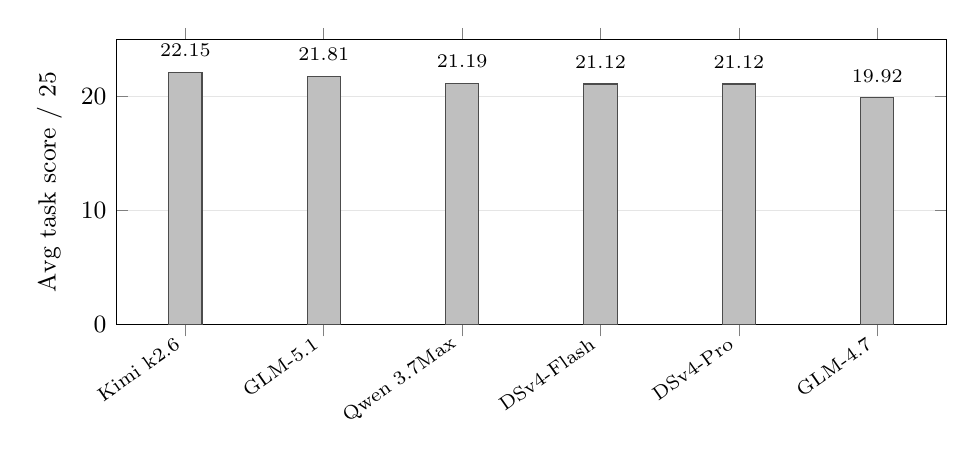
\begin{tikzpicture}
\begin{axis}[
    ybar,
    width=\columnwidth,
    height=5.2cm,
    ymin=0,
    ymax=25,
    ylabel={Avg task score / 25},
    symbolic x coords={Kimi,GLM5,Qwen,DSF,DSP,GLM4},
    xtick=data,
    xticklabels={Kimi k2.6,GLM-5.1,Qwen 3.7Max,DSv4-Flash,DSv4-Pro,GLM-4.7},
    x tick label style={rotate=35,anchor=east,font=\scriptsize},
    ymajorgrids=true,
    grid style={gray!20},
    nodes near coords,
    every node near coord/.append style={font=\scriptsize, anchor=south, yshift = 2 pt},
    bar width=12pt,
    tick label style={font=\small},
    label style={font=\small}
]
\addplot[fill=black!25,draw=black!70] coordinates {
    (Kimi,22.154)
    (GLM5,21.808)
    (Qwen,21.192)
    (DSF,21.115)
    (DSP,21.115)
    (GLM4,19.923)
};
\end{axis}
\end{tikzpicture}
\caption{Average task score by model. The high absolute scores motivate the saturation analysis rather than a strong leaderboard-style claim.}
\label{fig:model-bars}
\end{figure}

\subsection{External Benchmark Context}

As model-selection context, public model cards and benchmark pages report strong results for these model families on knowledge, mathematical reasoning, coding, and software-engineering benchmarks. Table~\ref{tab:external-context} summarizes the public scores collected in our model-audit sheet and places them next to the \pimplanbench{} average task score. These external results are included only as context. They come from heterogeneous protocols, have uneven coverage across model versions, and do not measure the planning-stage physics-informed modeling capability targeted by \pimplanbench{}.

\begin{table*}[t]
\caption{Public benchmark context for the evaluated models. The context mean is an unweighted average over available public entries in the audit sheet and is not used for PlanScore scoring or model ranking. Missing entries indicate that no clear public score was found for the exact model/benchmark/version. The DeepSeek-V4-Pro context row uses the public V4-Pro Max benchmark column available in the source sheet. LCB: LiveCodeBench; SWE-V: SWE-Bench Verified; MMLU-P: MMLU-Pro.}
\label{tab:external-context}
\centering
\scriptsize
\begin{tabular}{lrrrrrrrr}
\toprule
\textbf{Model} & \textbf{Public n} & \textbf{Ctx. mean} & \textbf{HLE} & \textbf{GPQA} & \textbf{LCB} & \textbf{SWE-V} & \textbf{MMLU-P} & \textbf{PIM (\%)} \\
\midrule
Kimi-K2.6 & \textbf{9} & 79.53 & 34.7 & 90.5 & 89.6 & 80.2 & 87.1 & \textbf{88.62} \\
GLM-5.1 & 7 & 74.76 & 31.0 & 86.2 & -- & -- & 86.0 & 87.23 \\
qwen3.7-max & 7 & 79.07 & \textbf{41.4} & \textbf{92.4} & 91.6 & 80.4 & -- & 84.77 \\
DeepSeek-V4-Flash & 1 & 68.30 & -- & -- & -- & -- & 68.3 & 84.46 \\
DeepSeek-V4-Pro & \textbf{9} & \textbf{80.62} & 37.7 & 90.1 & \textbf{93.5} & \textbf{80.6} & \textbf{87.5} & 84.46 \\
GLM-4.7 & 6 & 72.58 & 24.8 & 85.7 & 84.9 & 73.8 & 84.3 & 79.69 \\
\bottomrule
\end{tabular}
\end{table*}

Differences between these public-context scores and the \pimplanbench{} ordering support the benchmark's complementarity. DeepSeek-V4-Pro has the highest public-context mean in Table~\ref{tab:external-context}, but it is tied in \pimplanbench{} average task score with DeepSeek-V4-Flash and trails Kimi-K2.6 and GLM-5.1. Conversely, GLM-5.1 ranks second on \pimplanbench{} despite a lower public-context mean than qwen3.7-max and DeepSeek-V4-Pro. We therefore treat external leaderboard scores as evidence that the evaluated models are generally capable, not as substitutes for direct evaluation of physics-informed modeling plans.

\subsection{Facet Patterns}

Across all models, model choice and training strategy receive higher average scores than physics constraints and validation. This pattern suggests that LLMs often know how to name plausible architectures and optimizers, but they are less consistently specific about the governing constraints and physical diagnostics that make a plan credible. Figure~\ref{fig:facet-bars} shows average facet scores. The readiness audit additionally reports that Model Choice has the highest ceiling rate at 57.7\%, while Physics Constraints has a lower mean score and ceiling rate. This indicates that future task revisions should target constraint-level specificity and validation diagnostics, not only architectural selection.

\begin{figure}[t]
\centering
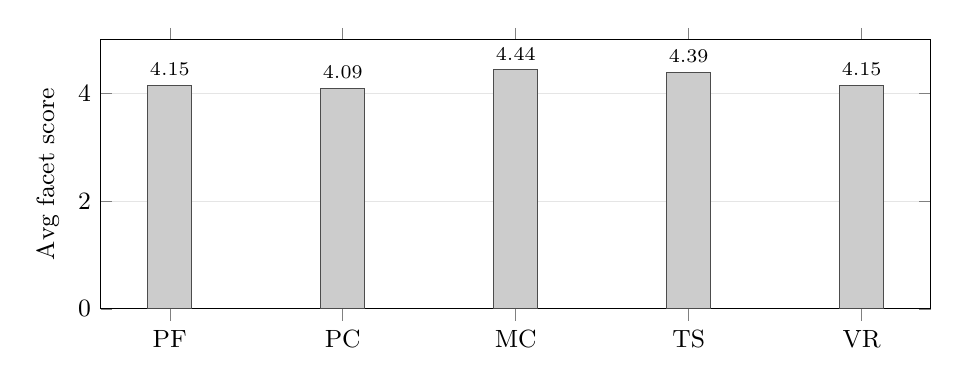
\begin{tikzpicture}
\begin{axis}[
    ybar,
    width=\columnwidth,
    height=5.0cm,
    ymin=0,
    ymax=5,
    ylabel={Avg facet score},
    symbolic x coords={PF,PC,MC,TS,VR},
    xtick=data,
    nodes near coords,
    every node near coord/.append style={font=\scriptsize},
    ymajorgrids=true,
    grid style={gray!20},
    bar width=16pt,
    tick label style={font=\small},
    label style={font=\small}
]
\addplot[fill=black!20,draw=black!70] coordinates {(PF,4.15) (PC,4.09) (MC,4.44) (TS,4.39) (VR,4.15)};
\end{axis}
\end{tikzpicture}
\caption{Average facet scores across the six-model pilot. PF: problem formalization; PC: physics constraints; MC: model choice; TS: training strategy; VR: validation and failure risks.}
\label{fig:facet-bars}
\end{figure}

\subsection{Saturation and Discrimination}

The readiness audit reports that 297 of 780 facet scores are exact 5.0 scores, giving a ceiling rate of 38.1\%. It also identifies 14 tasks with task-score range at most 3.0 and 28 task-facet groups with range at most 0.5. These diagnostics matter because the benchmark is intended to distinguish planning quality, not merely confirm that models can produce plausible structured prose.

The highest-separation tasks are informative. Compressible Euler shocks and divergence-controlled MHD show task-score ranges of 8.0 and 7.0, respectively, because they force central mathematical decisions. In contrast, hard-plus Helmholtz staircase and acoustic-scattering maze tasks show range 1.0, suggesting that their public prompts or private cap rules may not yet force enough model-specific choices. This is a useful benchmark-development signal: low-discrimination tasks should be rewritten or rescored with stricter critical points before \pimplanbench{} is used as a leaderboard.

\subsection{Human Calibration}

The current repository includes two v0.3 manual comparison workbooks covering 180 rows. Table~\ref{tab:manual-auto} summarizes the comparison. The automatic scorer has mean absolute difference 0.442 from human scores, 78.3\% within 0.5, and 96.7\% within 1.0. The largest discrepancy is in Problem Formalization, where the human mean is 4.569 and the automatic mean is 4.000. This indicates that the automatic scorer is conservative in some formulation cases, especially when a model correctly identifies the phenomenon but the keyword-based matching under-recognizes conditional missing-information handling.

\begin{table}[t]
\caption{Manual-auto calibration on 180 rows from selected v0.3 workbooks. The automatic scorer is useful for screening, but paper-facing claims should remain human-checked.}
\label{tab:manual-auto}
\centering
\small
\begin{tabular}{lr}
\toprule
\textbf{Metric} & \textbf{Value} \\
\midrule
Compared rows & 180 \\
Human mean & 4.381 \\
Automatic mean & 4.278 \\
Mean human minus auto & 0.103 \\
Mean absolute difference & 0.442 \\
Exact match rate & 0.378 \\
Within 0.5 rate & 0.783 \\
Within 1.0 rate & 0.967 \\
\bottomrule
\end{tabular}
\end{table}

\section{Discussion}

\pimplanbench{} shows that planning-stage physics-informed modeling is a measurable and useful NLP evaluation target. The pilot models produce complete structured plans, but high fluency does not guarantee task-specific correctness. Many answers score well because they mention plausible PINN components, optimizers, and validation ideas. The hard-trap cases show why explicit cap rules are necessary: planning quality depends on whether the answer handles the central mathematical difficulty, such as shocks, high-frequency phase, divergence-free fields, mass conservation, multiscale flux continuity, or missing specifications.

The benchmark also demonstrates a practical evaluation loop. Ceiling rate and model separation identify saturated tasks. Human-auto differences identify scoring rules that are too strict, too permissive, or too keyword-dependent. Private references can then be revised with sharper critical points and cap rules. This iterative loop is important for a compact benchmark, because the goal is not only to rank models but to diagnose which aspects of planning-stage scientific reasoning remain weak.

For EMNLP, the benchmark contributes a language-centered evaluation of domain-grounded planning under structured output constraints. For AI4Science, it provides a lightweight audit stage before expensive execution: a plan that cannot identify knowns and unknowns, physics constraints, or validation risks is unlikely to become a reliable solver through code generation alone.

\section{Reproducibility}

All benchmark artifacts are version-controlled to support reproducibility and auditability. The repository contains the public task set, the private reference set with cap rules, the general rubric, normalized model outputs, scored results and summaries, manual--automatic comparison outputs, and readiness-audit materials. The accompanying implementation covers task execution, output normalization, row construction, deterministic first-pass scoring, visualization, manual-review workbook generation, manual--automatic comparison, and readiness auditing.

The scoring and audit pipeline uses repository-local scripts rather than external NLP evaluation packages such as ROUGE, BLEU, NLTK, or spaCy. The request-level evaluation parameters are reported in Table~\ref{tab:api-config}, and the repository documents the script entry points needed to reproduce the pipeline.

The public task file, code, scoring summaries, and review workbooks are intended for research, reproduction, and benchmark-audit use. The private reference file is included to make scoring auditable but is not intended to be used as a model-facing prompt, training target, or leaderboard-tuning resource; the public release will include explicit license and access metadata for each artifact class.

The benchmark tasks and private references are author-constructed technical physics prompts rather than text collected from human subjects or social platforms. We manually reviewed the public and private task records for names, unique personal identifiers, and offensive content, and also checked the repository artifacts for obvious contact-information patterns before release. The released benchmark artifacts are not intended to contain personally identifying information; any provider-specific credentials or local configuration values are excluded from release.

\section*{Limitations}

The current v0.3 release is a compact pilot rather than a large-scale benchmark. It contains 26 tasks, which is enough for diagnostic analysis but not enough for broad claims about all scientific reasoning. The current scoring pipeline includes deterministic first-pass scoring and a 180-row manual calibration subset, but full inter-annotator agreement has not yet been reported. Execution validation is also not yet implemented as a systematic experiment. Therefore, the numerical results should be framed as direct-planner pilot evidence and not as final model rankings.

The benchmark focuses on planning-stage physics-informed modeling. It does not evaluate whether a generated plan can be implemented without errors, whether a trained neural solver converges, or whether a downstream agent can manage simulation tools. These are important but distinct targets. Future versions should add execution-validation subsets for tasks with analytic or trusted numerical references, expand human adjudication, and include deliberately weaker baselines to improve ranking discrimination.

The public benchmark context in Table~\ref{tab:external-context} is not a controlled cross-benchmark comparison. It is collected from public model cards and benchmark pages with uneven metric coverage, so it should only be used to contextualize model selection rather than to support statistical claims about model capability.

\section*{Ethics Statement}

\pimplanbench{} evaluates language-model planning for scientific modeling workflows. It should not be used as evidence that a model can autonomously solve PDEs, validate simulations, or replace domain experts. The private references include hidden scoring criteria to reduce overfitting and leakage, but any public release should clearly distinguish public prompts from private scoring files.

The manual calibration subset reported in Section~6.5 consists of internal review of model-output rows using the same scoring rubric and released review workbooks described in Section~8 and Appendix~\ref{app:rubric-details}. No external crowdworkers, students, or other human-subject participants were recruited or paid, and no personal or demographic data about annotators are collected or released. The annotation target is model output for technical physics tasks, not data about identifiable people.

General-purpose AI assistants were used for code organization support, table preparation, and language editing during manuscript preparation. The authors reviewed all generated suggestions and remain responsible for the scientific claims, experiments, scoring decisions, and final text.

\bibliographystyle{acl_natbib}
\bibliography{custom}

\appendix

\section{Benchmark Task Inventory}
\label{app:task-inventory}

Table~\ref{tab:full-task-inventory} lists all 26 public tasks in \pimplanbench{} v0.3. Task identifiers match the records in \texttt{dataset/tasks\_public\_v0.3.jsonl}; domain and task-type labels are rendered with spaces for readability.

\begin{table*}[t]
\caption{Complete v0.3 task inventory.}
\label{tab:full-task-inventory}
\centering
\scriptsize
\begin{tabularx}{\textwidth}{@{}p{0.31\textwidth}p{0.08\textwidth}p{0.15\textwidth}p{0.21\textwidth}X@{}}
\toprule
\textbf{Task ID} & \textbf{Diff.} & \textbf{Domain} & \textbf{Task type} & \textbf{PDE/system} \\
\midrule
\texttt{easy\_heat\_1d\_dirichlet\_001} & easy & heat transfer & forward PDE solving & 1D heat equation \\
\texttt{easy\_wave\_1d\_icbc\_002} & easy & wave propagation & forward PDE solving & 1D wave equation \\
\texttt{easy\_poisson\_2d\_source\_003} & easy & potential fields & forward PDE solving & 2D Poisson equation \\
\texttt{easy\_burgers\_1d\_periodic\_004} & easy & fluid dynamics & forward PDE solving & 1D viscous Burgers equation \\
\texttt{easy\_advection\_1d\_periodic\_005} & easy & transport & forward PDE solving & 1D linear advection equation \\
\texttt{easy\_reaction\_diffusion\_1d\_006} & easy & chemical biology & forward PDE solving & 1D reaction-diffusion equation \\
\texttt{easy\_laplace\_2d\_boundary\_007} & easy & potential fields & boundary value problem & 2D Laplace equation \\
\texttt{medium\_advection\_diffusion\_008} & medium & transport & forward PDE solving & Advection-diffusion equation \\
\texttt{medium\_heat\_inverse\_alpha\_009} & medium & heat transfer & inverse parameter estimation & 1D heat equation \\
\texttt{medium\_burgers\_inverse\_viscosity\_010} & medium & fluid dynamics & inverse parameter estimation & 1D viscous Burgers equation \\
\texttt{medium\_poisson\_source\_recovery\_011} & medium & potential fields & unknown source recovery & 2D Poisson equation \\
\texttt{medium\_wave\_sparse\_sensors\_012} & medium & wave propagation & sparse observation modeling & 1D wave equation \\
\texttt{medium\_reaction\_diffusion\_noisy\_013} & medium & chemical biology & noisy data fitting & Two-species reaction-diffusion system \\
\texttt{medium\_heat\_mixed\_bc\_014} & medium & heat transfer & boundary condition handling & 1D heat equation \\
\texttt{medium\_periodic\_advdiff\_015} & medium & transport & periodic constraint handling & Periodic advection-diffusion equation \\
\texttt{hard\_allen\_cahn\_016} & hard & phase field & stiff phase-field modeling & Allen-Cahn equation \\
\texttt{hard\_cahn\_hilliard\_017} & hard & phase field & high-order PDE modeling & Cahn-Hilliard equation \\
\texttt{hard\_navier\_stokes\_2d\_018} & hard & fluid dynamics & forward or data assimilation & 2D incompressible Navier-Stokes equations \\
\texttt{hard\_darcy\_heterogeneous\_019} & hard & porous media & heterogeneous coefficient field & Darcy flow \\
\texttt{hard\_helmholtz\_high\_frequency\_020} & hard & wave physics & high-frequency frequency-domain modeling & Helmholtz equation \\
\texttt{hard\_plus\_helmholtz\_staircase\_021} & hard+ & wave physics & complex-geometry high-frequency modeling & High-frequency Helmholtz equation in staircase geometry \\
\texttt{hard\_plus\_acoustic\_scattering\_maze\_022} & hard+ & acoustics & complex-geometry scattering & Acoustic scattering in maze-like geometry \\
\texttt{hard\_plus\_euler\_shock\_023} & hard+ & compressible flow & discontinuous solution modeling & Compressible Euler equations with shocks \\
\texttt{hard\_plus\_rayleigh\_benard\_024} & hard+ & thermal-fluid dynamics & coupled multiphysics modeling & Rayleigh-Benard convection under Boussinesq approximation \\
\texttt{hard\_plus\_mhd\_divergence\_025} & hard+ & magnetohydrodynamics & coupled divergence-free field modeling & Resistive magnetohydrodynamics \\
\texttt{hard\_plus\_multiscale\_darcy\_026} & hard+ & porous media & multiscale operator or solver design & Multiscale Darcy flow with high-contrast permeability \\
\bottomrule
\end{tabularx}
\end{table*}

\section{Scoring Rubric Details}
\label{app:rubric-details}

This appendix summarizes the public scoring guidance used by \planscore{} v0.3. The private reference file contains task-specific critical points and acceptable alternatives, but the scoring principles below are sufficient to interpret the reported pilot scores. Tables~\ref{tab:appendix-score-scale} and~\ref{tab:appendix-facet-full-credit} summarize the score scale and facet-specific full-credit patterns, while Tables~\ref{tab:appendix-general-caps} and~\ref{tab:appendix-hard-trap-caps} give general and hard-trap cap examples.

\begin{table*}[t]
\caption{General interpretation of the 0--5 \planscore{} facet scale.}
\label{tab:appendix-score-scale}
\centering
\small
\begin{tabularx}{\textwidth}{@{}p{0.08\textwidth}X@{}}
\toprule
\textbf{Score} & \textbf{General interpretation} \\
\midrule
0 & Missing, irrelevant, unmappable to the required facet, or physically incompatible with the task. \\
1 & Recognizes the broad phenomenon or repeats the prompt, but lacks a usable formulation, constraint, model, training plan, or validation plan. \\
2 & Partially correct, but with major omissions such as missing variables, conditions, data terms, task type, or core physical assumptions. \\
3 & Basic task-aware answer with the main workflow component present, but still generic, incomplete, or missing important execution details. \\
4 & Strong answer that is mostly task-specific and operational, with at most one important subtlety, risk, or execution detail missing. \\
5 & Complete, task-specific, executable, and risk-aware answer that satisfies the relevant critical points without triggering a cap rule. \\
\bottomrule
\end{tabularx}
\end{table*}

\begin{table*}[t]
\caption{Facet-specific full-credit criteria used to guide human review and interpret automatic scores.}
\label{tab:appendix-facet-full-credit}
\centering
\small
\begin{tabularx}{\textwidth}{@{}p{0.20\textwidth}X@{}}
\toprule
\textbf{Facet} & \textbf{Full-credit pattern} \\
\midrule
Problem Formalization & Separates known inputs, unknown fields, inferred parameters, domain or geometry, data roles, missing specifications, and forward/inverse/data-assimilation/surrogate objective without inventing unsupported details. \\
Physics Constraints & States the governing residuals and the relevant IC, BC, observation, conservation, compatibility, divergence, periodicity, source, or material constraints in a task-specific way. \\
Model Choice & Selects a model family and architecture that match the PDE type, data regime, geometry, regularity, frequency, conservation structure, identifiability, or intended generalization setting. \\
Training Strategy & Defines losses, sampling regions, weighting, normalization, optimizer schedule, stabilization, and monitoring criteria that address the main difficulty of the task. \\
Validation Failure Risks & Reports task-specific metrics and failure modes, such as residual maps, IC/BC error, held-out data consistency, conservation or flux error, divergence error, phase error, shock location, energy drift, or identifiability checks. \\
\bottomrule
\end{tabularx}
\end{table*}

\begin{table*}[t]
\caption{General cap rules in \planscore{} v0.3. Caps are applied after reading the answer for the affected facet; when multiple caps apply, the strictest cap is used.}
\label{tab:appendix-general-caps}
\centering
\scriptsize
\begin{tabularx}{\textwidth}{@{}p{0.23\textwidth}p{0.12\textwidth}X@{}}
\toprule
\textbf{Condition} & \textbf{Cap} & \textbf{Rationale} \\
\midrule
Generic PINN template & $\leq 3$ & A broadly plausible PINN recipe should not receive full credit without task-specific residuals, constraints, model rationale, training details, or risks. \\
Hallucinated specifications & $\leq 2$ & Concrete ICs, BCs, parameter values, geometries, coefficient fields, sensor layouts, or source terms not in the public prompt must be labeled as assumptions. \\
Method name without execution detail & $\leq 2$ & Naming PINN, FNO, DeepONet, SIREN, weak form, vector potential, or domain decomposition is insufficient without inputs, outputs, losses, sampling, training, and validation. \\
Wrong task type & $\leq 2$ & Treating a forward problem as inverse, or an inverse/data-assimilation problem as a pure forward solve, changes the required workflow. \\
Wrong PDE type or physics & $\leq 2$ & Replacing the governing equation class, such as treating Helmholtz as a time-domain wave equation or Cahn-Hilliard as Allen-Cahn, invalidates key facets. \\
Missing required data term & $\leq 2$ & If observations or sparse measurements are public, omitting the data-misfit term removes a central part of the objective. \\
Missing central IC, BC, or constraint & $\leq 3$ or $\leq 2$ & Omitted public conditions or constraints cap affected Physics Constraints and Training Strategy facets; the stricter cap is used when the missing term is central. \\
Validation only uses MSE & $\leq 3$ & Generic field MSE is insufficient without physical checks such as residual, IC/BC error, conservation, divergence, phase, flux, shock, or data consistency. \\
Schema violation & 0 for missing facets & If an answer cannot be mapped to the required five facets, unmappable facets are scored as missing unless a faithful manual mapping is documented. \\
\bottomrule
\end{tabularx}
\end{table*}

\begin{table*}[t]
\caption{Examples of hard-trap cap rules. These examples illustrate how task-specific scoring prevents generic answers from receiving full credit.}
\label{tab:appendix-hard-trap-caps}
\centering
\scriptsize
\begin{tabularx}{\textwidth}{@{}p{0.27\textwidth}p{0.18\textwidth}X@{}}
\toprule
\textbf{Task ID} & \textbf{Affected facets} & \textbf{Example cap condition} \\
\midrule
\texttt{medium\_periodic\_advdiff\_015} & Physics Constraints, Training Strategy, Validation Failure Risks & Fixed Dirichlet endpoint treatment is capped at 2 for affected constraints and training; value-only periodicity without derivative or diffusive-flux compatibility is capped at 3. \\
\texttt{hard\_cahn\_hilliard\_017} & Problem Formalization, Physics Constraints, Model Choice, Training Strategy, Validation Failure Risks & Treating Cahn-Hilliard as Allen-Cahn is capped at 2 on formulation, constraints, and model choice; omitting chemical potential or fourth-order burden caps model and training at 3. \\
\texttt{hard\_helmholtz\_high\_frequency\_020} & Problem Formalization, Physics Constraints, Model Choice, Training Strategy, Validation Failure Risks & Treating Helmholtz as time-domain wave propagation is capped at 2 on formulation and constraints; naming Fourier features or SIREN without complex, wavelength, or phase detail is capped at 3. \\
\texttt{hard\_plus\_euler\_shock\_023} & All facets except where inapplicable & A smooth strong-form pointwise PINN without weak, integral, conservative, or shock-aware treatment caps model, training, and validation at 2; omitting conservation form caps formulation and constraints at 2. \\
\texttt{hard\_plus\_mhd\_divergence\_025} & Problem Formalization, Physics Constraints, Model Choice, Training Strategy, Validation Failure Risks & Omitting magnetic divergence control caps affected physics, model, and validation facets at 2; relying only on a soft divergence penalty without constrained parameterization, projection, or drift validation is capped at 3. \\
\texttt{hard\_plus\_multiscale\_darcy\_026} & Problem Formalization, Physics Constraints, Model Choice, Training Strategy, Validation Failure Risks & Failing to distinguish a single high-contrast solve from reusable surrogate/operator learning caps formulation, model, and training at 3; ignoring high-contrast effects, flux continuity, or mass balance caps affected facets at 2. \\
\bottomrule
\end{tabularx}
\end{table*}

\end{document}
